%class
	\documentclass{beamer}

%template
	\usetheme{HannoverSalman}
	\setbeamertemplate{navigation symbols}{}
	%\setbeamertemplate{footline}{\centering{\insertframenumber/\insertpresentationendpage}}
	%\setbeamertemplate{footline}{\hspace*{.5cm}\scriptsize{\hfill\insertframenumber\hspace*{.5cm}}} 


%packages
	\usepackage{amsmath, amssymb, graphicx,cancel}
	\usepackage[absolute,overlay]{textpos}
	\usepackage{subfigure}
	\usepackage{caption}\captionsetup{labelformat=empty,labelsep=none}
	\usepackage{geometry}
	\geometry{verbose}
	\usepackage{color}
	\usepackage{xmpmulti}
	\usepackage[3D]{movie15}
	\usepackage{hyperref}
%	\usepackage{bookmark}
	\usepackage[open,openlevel=4,atend]{bookmark}
	%\bookmarksetup{color=blue}
	\usepackage{multirow}
	\usepackage[style=numeric,defernumbers, authoryear]{biblatex}
	%\usepackage[square,sort]{natbib}
	%\usepackage{fancyhdr}%\pagestyle{fancy} 

	
	\hypersetup{bookmarksdepth = 4}


%citations files
	\bibliography{MyCitations}

%logoCSIPCPL
    \setlength{\TPHorizModule}{1mm}
    \setlength{\TPVertModule}{1mm}
    \newcommand{\logoCSIPCPL}
    {
    	\begin{textblock}{1}(100,2) %(100,85)  for bottom
    		
\includegraphics[width=1.5cm]{figs/logo_CSIP}
    	\end{textblock}
    	
	\begin{textblock}{1}(117,1) %(117,85)  for bottom
    		
\includegraphics[width=1.0cm]{figs/logo_CPL}
    	\end{textblock} 
    }

%logo evolution
    \newcommand{\logoEvolution}
    {    	
	\begin{textblock}{1}(110,1) %(117,85)  for bottom
    		\includegraphics[width=0.65in]{figs/logo_evolution.pdf}
    	\end{textblock} 
    }

%logo Qualcomm
    \newcommand{\logoQualcomm}
    {
    	\begin{textblock}{1}(110,2) %(100,85)  for bottom
    		\includegraphics[width=1.5cm]{figs/logo_qualcomm.jpg}
    	\end{textblock}
    }
%logo Qualcomm (long)
    \newcommand{\logoQualcommllong}
    {
    	\begin{textblock}{1}(0,0) 
    		\includegraphics[width=1.25in]{figs/logo_qualcomm_long.jpg}
    	\end{textblock}
    }

%logo Tech Tower
    \newcommand{\logoTechTower}
    {
    	\begin{textblock}{1}(0,0) 
    		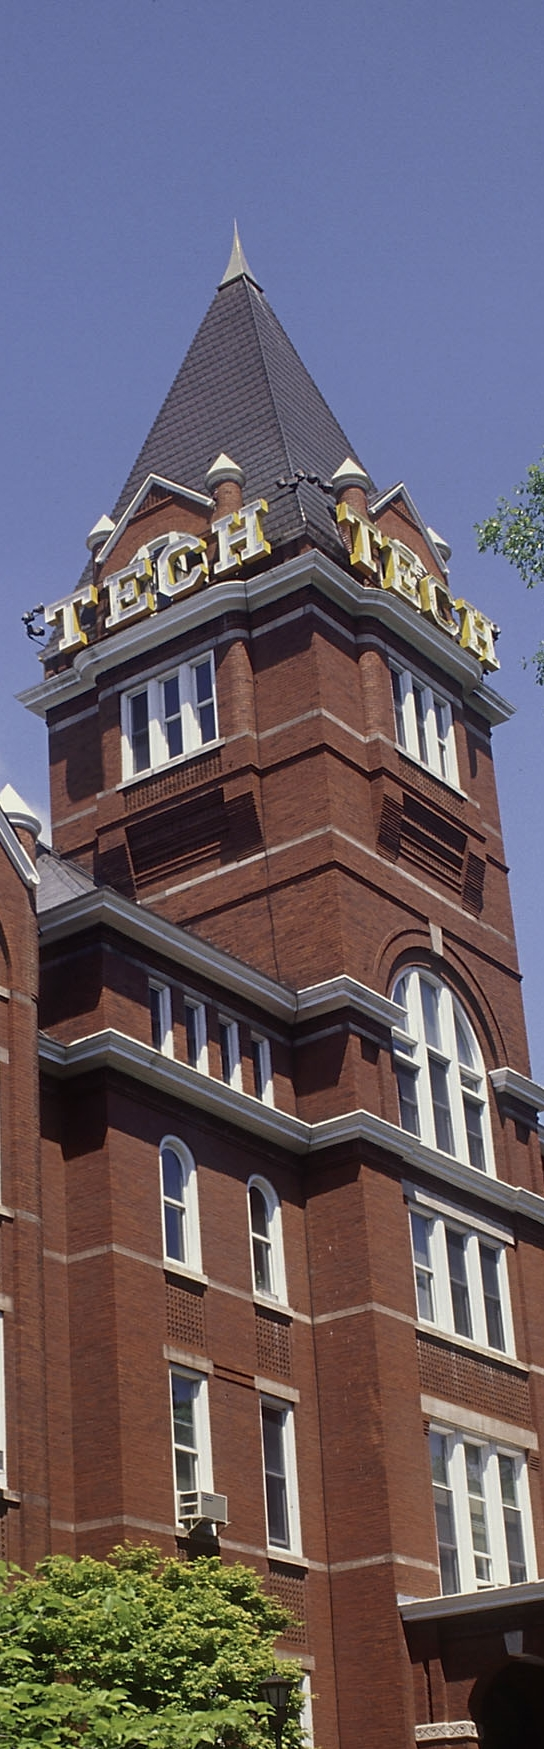
\includegraphics[width=1.25in]{figs/logo_TechTower.jpg}
    	\end{textblock}
    }

%logo tree
    \newcommand{\logoTree}
    {
    	\begin{textblock}{1}(0,0) 
    		\includegraphics[width=1.25in]{figs/logo_tree.jpg}
    	\end{textblock}
    }
%page numbers
    \newcommand{\mypagenum}
    {
    	\begin{textblock}{1}(1,94) 
		{\tiny \color[rgb]{0.2,0.2,1}\insertframenumber} %\insertframenumber,\insertpresentationendpage, \inserttotalframenumber
    	\end{textblock}
    }
%my footnote citation
	\newcommand{\myFootnoteCitation}[2]
	{
		\footnote{\tiny \citeauthor{#1}, \emph{#2}, \citeyear{#1}.}  %\citeauthor{#1}, \citetitle{#1}, #2 \citeyear{#1}.
	}
%my refer to citation
	\newcommand{\mycite}[1]
	{
		\emph{\citeauthor{#1} (\citeyear{#1})}
	}
%my footnote website citation
	\newcommand{\myFootnoteWebsiteCitation}[1]
	{
		\footnote{\tiny \citeauthor{#1}}
	}

\let\thefootnote\relax\footnotetext{Footnotetext without footnote mark}


%section underline
%\newcommand{\tmpsection}[1]{}
%\let\tmpsection=\section
%\renewcommand{\section}[1]{\tmpsection{\underline{#1}}}



%commands
	\newcommand{\likelihood}{p(Z_k| x_k) }						%likelihood
	\newcommand{\prior}{p(x_k)  } 								%prior
	\newcommand{\posterior} {p(x_k| Z_k)}						%posterior
	\newcommand{\prediction} {p(x_k| Z_{k-1})}					%prediction
	\newcommand{\update} {p(x_k|Z_k)}							%update
	\newcommand{\observations} {p(Z_k)}						%observations
	\newcommand{\prevobservations} {p(Z_{k-1})}				%previous observations
	\newcommand{\dxpk} {dx_{k-1}}							%dx_{k-1}
	\newcommand{\ChapKolm}{\int{p(x_k| x_{k-1})p(x_{k-1}|Z_{k-1})} \dxpk} %Chapman Kolmogorov

	%algorithm specific: JPDAF
	\newcommand{\likelihoodJPDAF}{p(Z_k| \chi, m, Z_{k-1}) }		%1. likelihood
	\newcommand{\priorJPDAF}{p(\chi|m, Z^{k-1}} 				%2. prior	
	\newcommand{\observationsJPDAF} {p(Z_k}					%3. observations
	\newcommand{\posteriorJPDAF} {p(\chi| Z_k)}					%4. posterior

%environments
	\newenvironment{changemargin}[2]
	{
	  	\begin{list}{}
		{
			\setlength{\topsep}{0pt}%
			\setlength{\leftmargin}{#1}%
			\setlength{\rightmargin}{#2}%
			\setlength{\listparindent}{\parindent}%
			\setlength{\itemindent}{\parindent}%
			\setlength{\parsep}{\parskip}%
		}
	  	\item[]
		}
		{\end{list}
	}
%figures

%colors
\definecolor{darkgreen}{rgb}{0,0.5,0}

%personal details
	\author{Salman Aslam}
	\institute{Advisor, Dr Christopher Barnes (ECE)\\Co-advisor, Dr Aaron Bobick (CoC)\\Georgia Institute of Technology}
	\date{}

\begin{document}
%####################################################################################################
\title{Visual Tracking}
%####################################################################################################
\begin{frame}[plain]\logoTechTower
	\titlepage
\end{frame}

\begin{frame}
\frametitle{Outline}
\logoCSIPCPL\logoTechTower
	\setcounter{tocdepth}{1}	
	\tableofcontents
\end{frame}

%#######################################################################
\section{INTRODUCTION}
%#######################################################################
\begin{frame}
\frametitle{Introduction}
\framesubtitle{definition}
\logoCSIPCPL\mypagenum
	Estimate and maintain {\color{red}target state} over {\color{red}time}
	\begin{figure}
		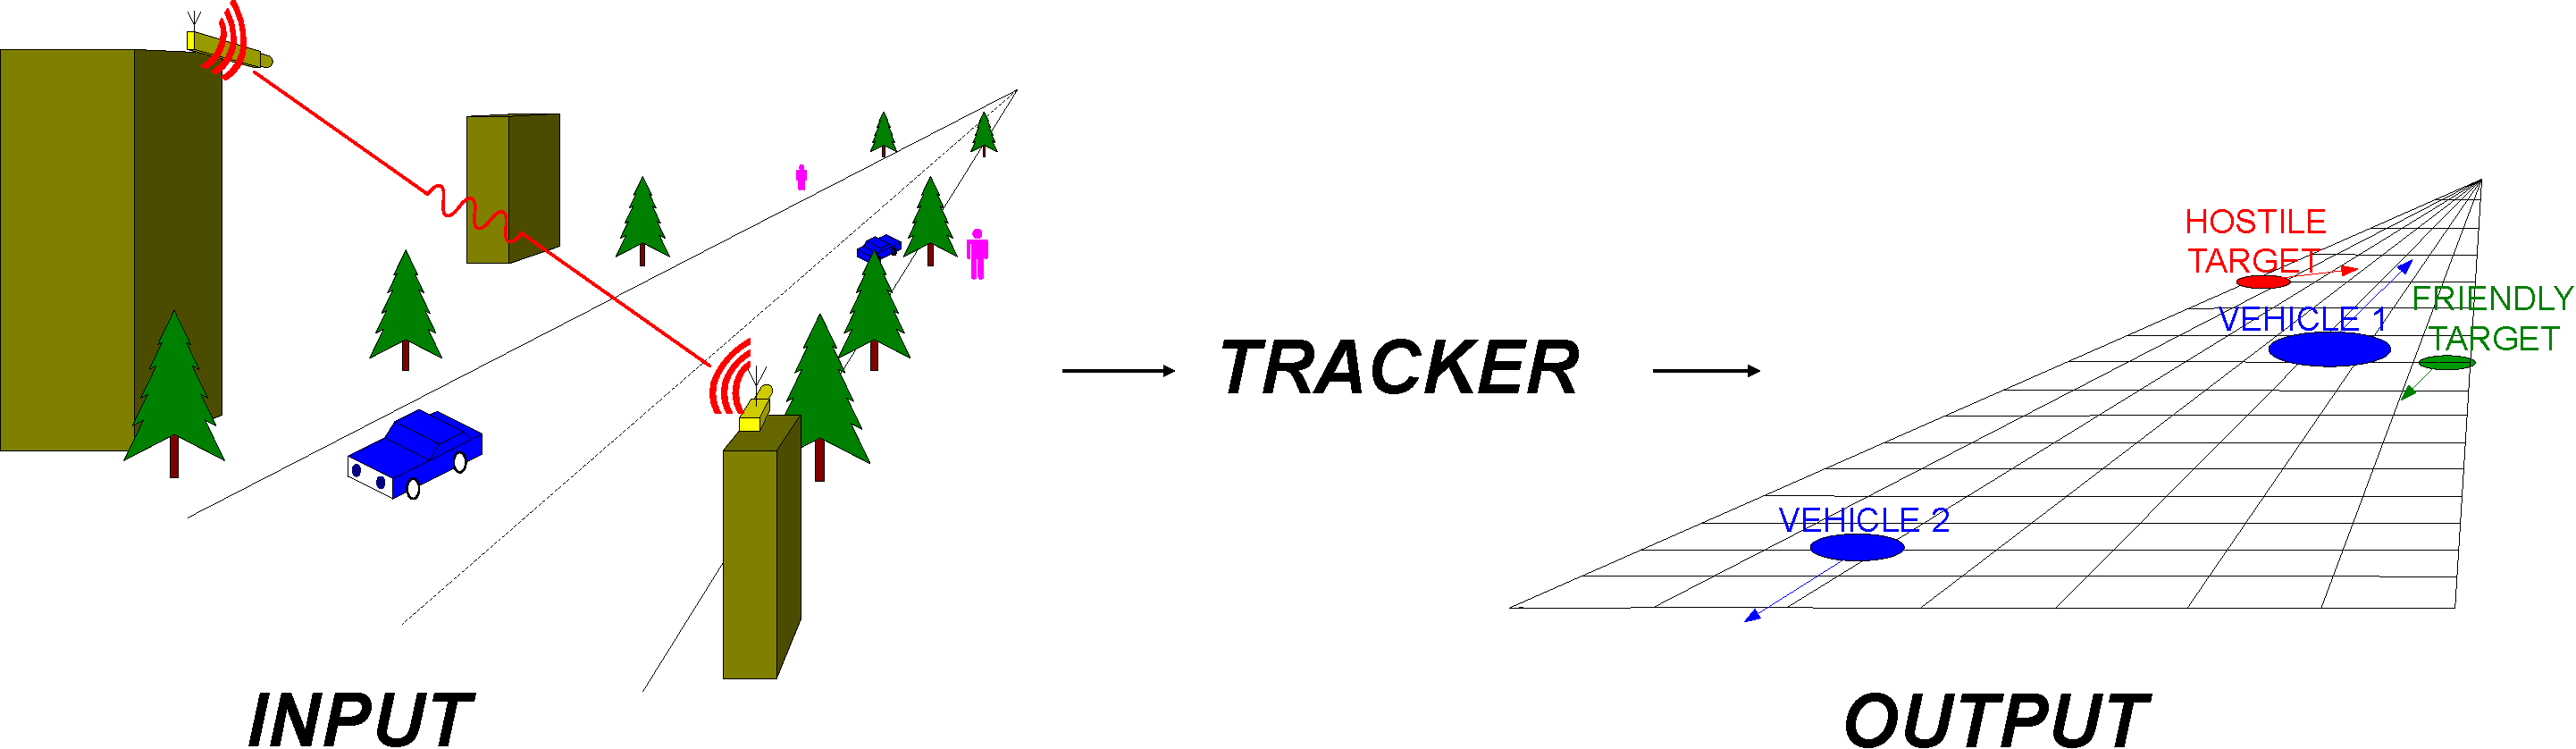
\includegraphics[width=1.0\textwidth]{figs/TRK_overviewDiagram.pdf}
	\end{figure}
\end{frame}

\begin{frame}[plain]
\frametitle{Introduction}
\framesubtitle{big picture}
\logoCSIPCPL\mypagenum
\myFootnoteCitation{2006_JNL_TrackingSurvey_Yilmaz}{ACM Computing Surveys}
	\begin{changemargin}{-1.35in}{0in}
		\begin{figure}
			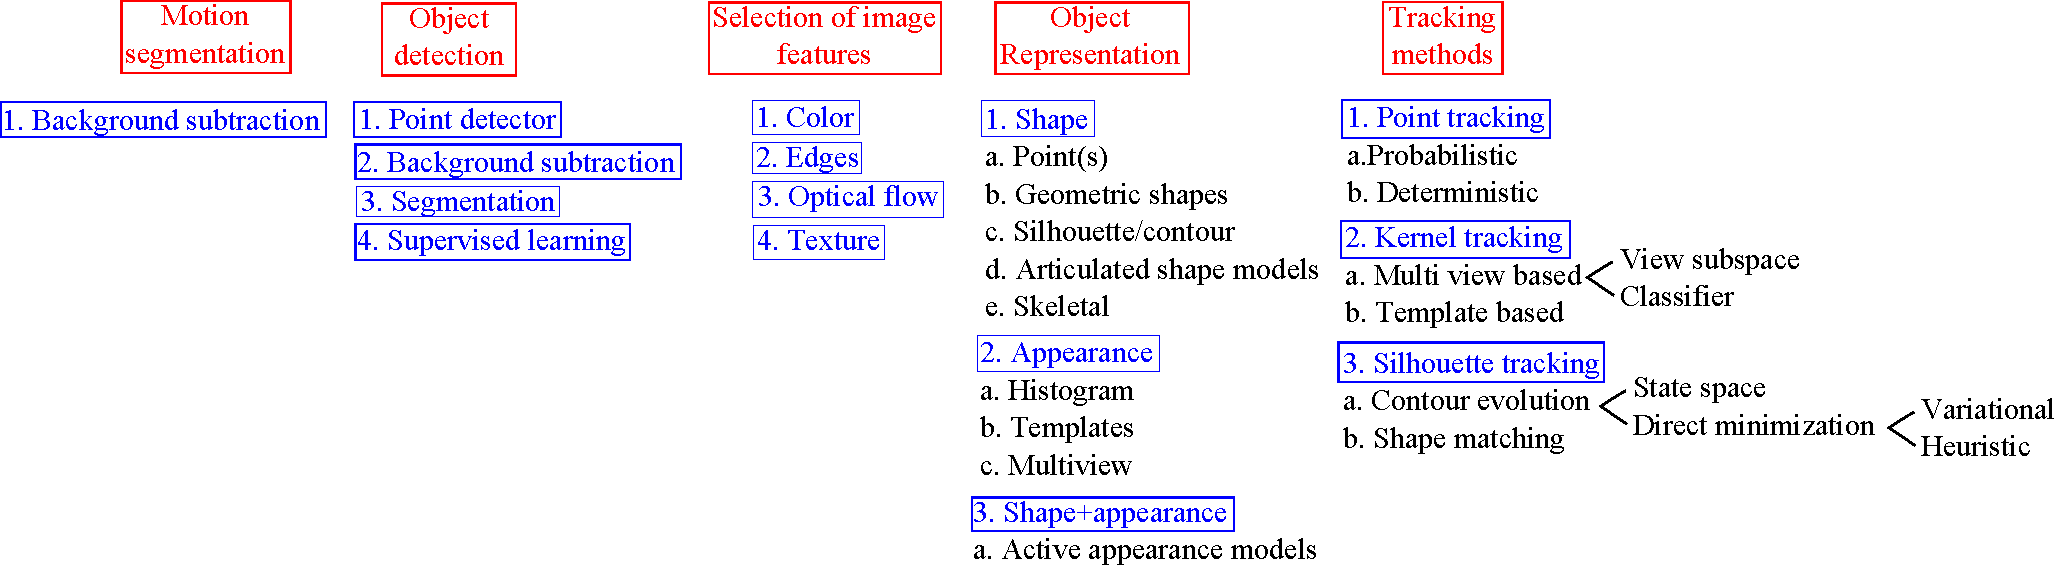
\includegraphics[width=1.35\textwidth]{figs/TRK_overview.pdf}
		\end{figure}	
	\end{changemargin}
\end{frame}



\begin{frame}
\frametitle{Introduction}
\framesubtitle{big picture: relation to PGMs}
\logoCSIPCPL\mypagenum
	\begin{figure}
		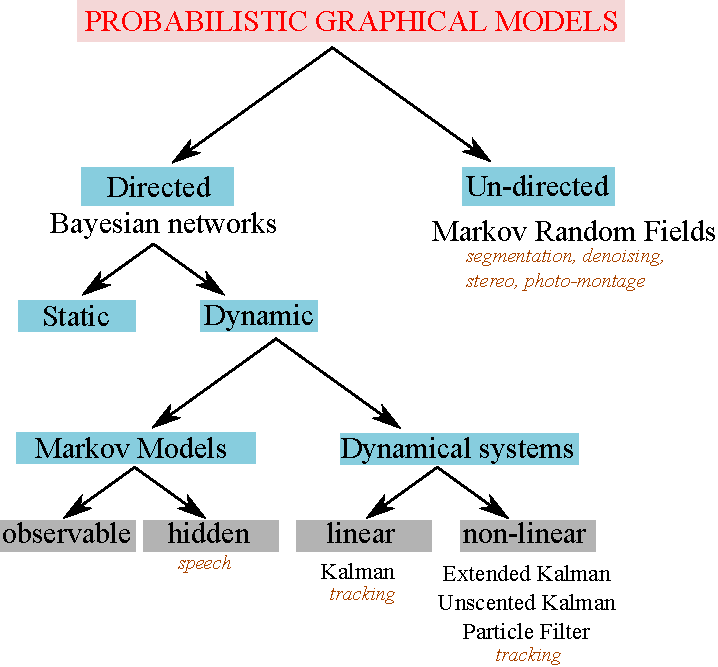
\includegraphics[width=0.9\textwidth]{figs/PRML_PGM_overview.pdf}
	\end{figure}
\end{frame}


\begin{frame}
\frametitle{Introduction}
\framesubtitle{big picture: relationship with HMM}
\logoCSIPCPL\mypagenum
	\begin{figure}
		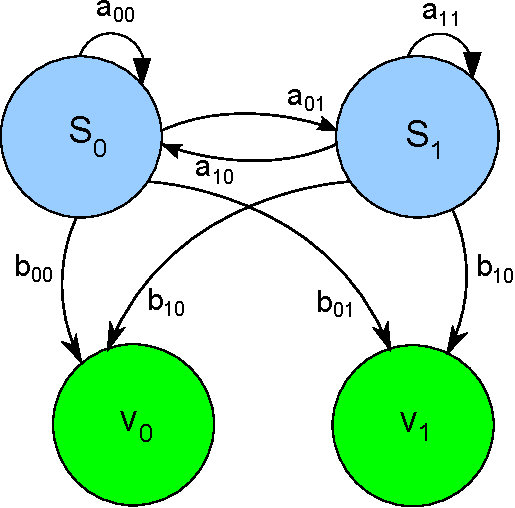
\includegraphics[height=0.3\textheight]{figs/HMM_flowDiagram.pdf}
	\end{figure}
	\begin{figure}
		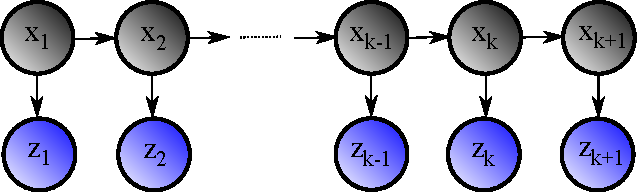
\includegraphics[width=1.0\textwidth]{figs/HMM_flowDiagram2.pdf}
	\end{figure}
\end{frame}




\begin{frame}
\frametitle{Introduction}
\framesubtitle{formulation: update}
\logoCSIPCPL\mypagenum
	\begin{figure}
		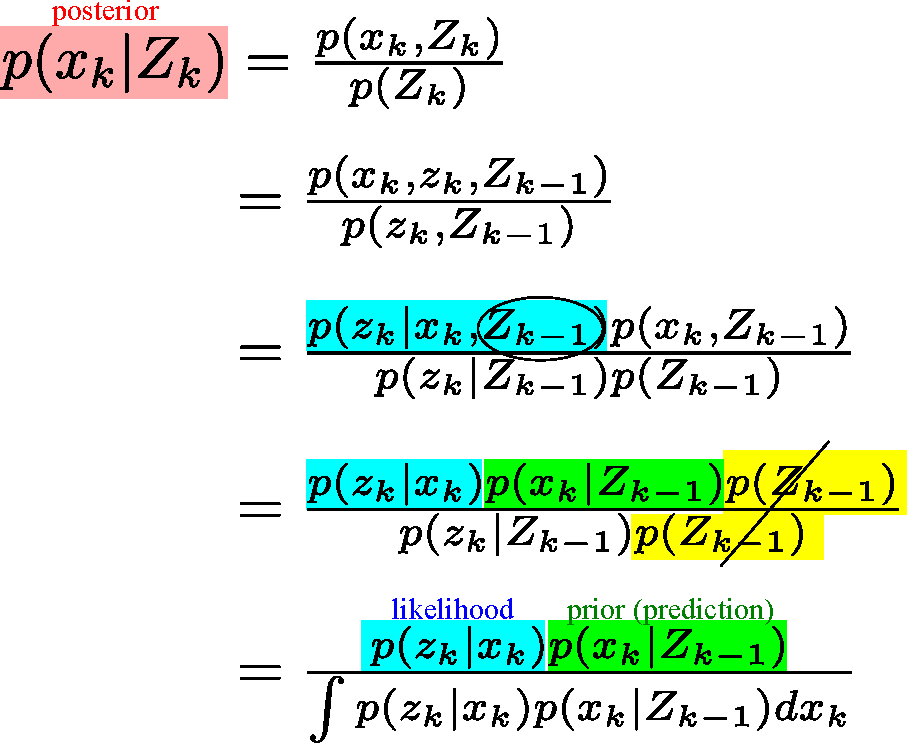
\includegraphics[width=1.0\textwidth]{figs/TRK_EQN_update.pdf}
	\end{figure}
\end{frame}



\begin{frame}
\frametitle{Introduction}
\framesubtitle{formulation: prediction}
\logoCSIPCPL\mypagenum
	Chapman Kolmogorov equation
	\begin{figure}
		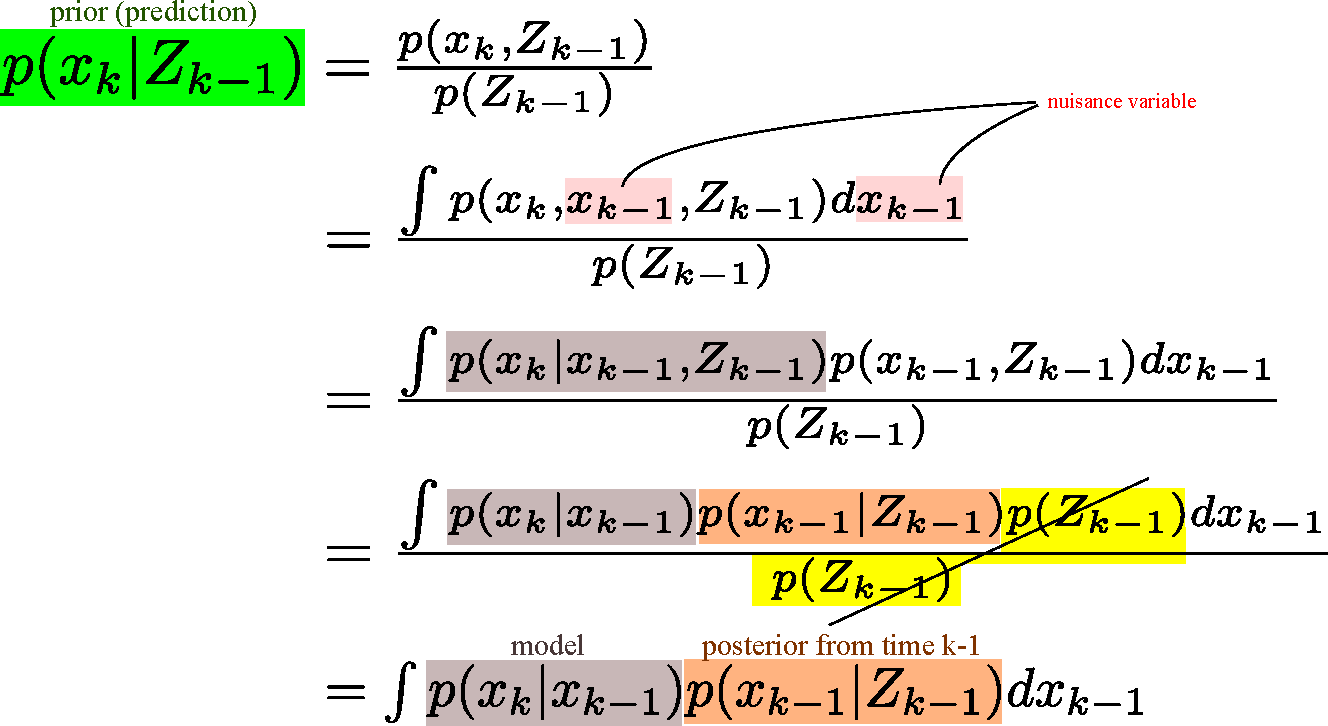
\includegraphics[width=1.0\textwidth]{figs/TRK_EQN_prediction.pdf}
	\end{figure}
\end{frame}


\begin{frame}
\frametitle{Introduction}
\framesubtitle{pre-processing: steps and features used}
\logoCSIPCPL\mypagenum
	{\color{red}Steps}
	\begin{enumerate}
		\item Downsampling
		\item Normalization
		\item Stabilization
		\item Background modeling
		\item Feature Extraction
	\end{enumerate}
	\vspace{0.1in}
	{\color{red}Features}
	\begin{enumerate}
		\item Color
		\item Edges
		\item Corners
		\item Motion
		\item Texture
		\item Depth
	\end{enumerate}
\end{frame}


\begin{frame}
\frametitle{Introduction}
\framesubtitle{pre-processing: depth using stereo}
\mypagenum
	\begin{figure}		
		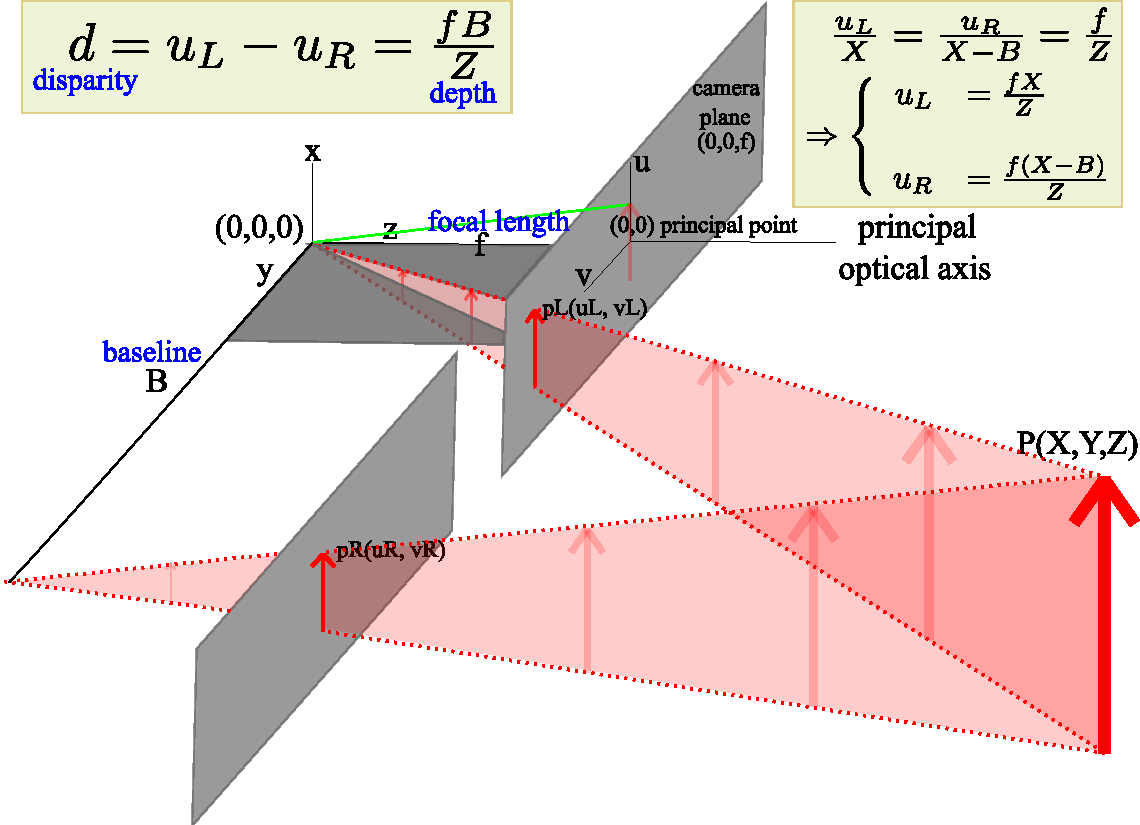
\includegraphics[width=1.0\textwidth]{figs/3D_2_cameras_blockDiagram.pdf}
	\end{figure}
\end{frame}	


\begin{frame}
\frametitle{Introduction}
\framesubtitle{types}
\logoCSIPCPL\mypagenum
	for more details, see tracking slides on point, appearance, contour, subspace, etc.
\end{frame}



%####################################################################################################
\section{PRIOR WORK}
%####################################################################################################
%==================================
\subsection{\ \ \ \ 2004: SURVEY (Dedeoglu)}
%==================================
\begin{frame}
\frametitle{Prior work: SURVEY (Dedeoglu)}
\framesubtitle{}
\mypagenum
\myFootnoteCitation{2004_MAS_SURVEYtrk_Dedeoglu}{Masters thesis, Bilkent University}
\end{frame}

%==================================
\subsection{\ \ \ \ 2006: SURVEY (Trucco)}
%==================================
\begin{frame}
\frametitle{Prior work: SURVEY (Trucco)}
\framesubtitle{}
\mypagenum
\myFootnoteCitation{2006_JNL_SURVEYtrk_Trucco}{OE}
\end{frame}



%==================================
\subsection{\ \ \ \ 2006: SURVEY (Yilmaz)}
%==================================
\begin{frame}
\frametitle{Prior work: SURVEY (Yilmaz)}
\framesubtitle{}
\mypagenum
\myFootnoteCitation{2006_JNL_SURVEYtrk_Yilmaz}{ACM Computing Surveys}
\end{frame}


%==================================
\subsection{\ \ \ \ 2008: SURVEY (Cannons)}
%==================================
\begin{frame}
\frametitle{Prior work: SURVEY (Cannons)}
\framesubtitle{}
\mypagenum
\myFootnoteCitation{2008_REP_SURVEYtrk_Cannons}{Technical report, York University}
\end{frame}




%####################################################################################################
\section{METHODOLOGY}
%####################################################################################################
\begin{frame}
\frametitle{Methodology}
\framesubtitle{steps: RVQ tracking}
\mypagenum
	\begin{enumerate}
		\item foreground extraction
			\begin{itemize}
				\item moving median background
		 		\item median filtering
				\item morphological close
				\item area thresholding
			\end{itemize}
		\item take one blob and extract 8x8 blocks centered on every 4th pixel in x and y directions
		\item save these blocks as class\_1\_example\_1.jpg, class\_1\_example\_2.jpg, class\_1\_example\_3.jpg and so on 
		\item train RVQ on these blocks to create a class conditional density for class 1.
		\item repeat this process for other blobs
		\item in the next frame, take a blob and compute idx's for all its blocks
		\item use a scalar XDR for maximum likelihood scoring of these blocks
	\end{enumerate}
\end{frame}



\begin{frame}
\frametitle{Methodology}
\framesubtitle{comparison 1: max likelihood using pixel based HS histogram}
\mypagenum
	\begin{itemize}
		\item appearance model is a color histogram similar to \mycite{2005_CNF_TRKoccl_Huang}
		\begin{itemize}
			\item histogram built over H and S channels in HSV color space
			\item H quantized into 16 bins
			\item S quantized into 8 bins
		\end{itemize}
	\end{itemize}
\end{frame}




\begin{frame}
\frametitle{Methodology}
\framesubtitle{comparison 2}
\mypagenum
	\begin{itemize}
		\item cut up target into 2 halves as in \mycite{2002_CNF_TRKcolor_Perez}		
			\begin{itemize}
				\item even if dividing line is not correct, I think this will work because dominant modes will be in their respective halves, and as you get more and more observations, they will be reinforced
				\item say a person is wearing different colored clothes
				\item instead of cutting exactly in the center, you include some shirt in pants
				\item shirt pixels in the trouser histogram will have small bin height, and will therefore not get picked when maximizing likelihood
			\end{itemize}
	\end{itemize}
\end{frame}


%####################################################################################################
\section{EXPERIMENTS}
%####################################################################################################



%####################################################################################################
\printbibliography
%####################################################################################################
%\bibliographystyle{ieee}
%\bibliography{c:/salman/work/writing/MyCitations}
\end{document}
%####################################################################################################

%####################################################################################################






























%- prune: if a certain position has no possible blobs, prune it
%- similarity: (a) correlation coefficient, (b) blob width, (c) blob height, (d) area

%metrics (2D vectors vs vertical position, take medians)
%(a) width (b) height (c) area


 
	%		\item "Hand-crafted" models	
	%			\begin{itemize}
	%				\item approach lacks generality
	%				\item new model for each application
	%			\end{itemize}
	%		\item Level sets, $\phi$ (implicit)
	%		\item finite element models
	%		\item Explicit: control points, $v$	

%
%
%Active Shape Models encompass a variety of forms, principally
%\emph{snakes}, \emph{deformable templates}, and \emph{dynamic
%contours}.
%
%
%%####################################################################################################
%\section{Snakes}
%%####################################################################################################
%A snake is an elastic contour which is fitted to features detected
%in an image.
%
%The nature of its elastic energy draws it more or less strongly to
%certain preferred configurations, representing prior information
%about shape which is to be balanced with evidence from an image.  If
%also inertia is attributed to a snake, it acquires dynamic behavior
%which can be used to apply prior knowledge of motion, not just of
%shape.
%
%Take a feature map $F(r)$, treat it like a landscape, and allow the
%snake, a deformable curve $r(s)$ to slither on it.  Equilibrium
%equations for r(s) are set up in such a way that r(s) tends to cling
%to high responses of $F$, that is, maximizing $F(r(s))$ over $0 \leq
%s \leq 1$, in some appropriate sense.  This tendency to maximize F
%is formalized as the "external" potential energy of the dynamical
%system.  It is counterbalanced by "internal" potential energy which
%tends to preserve smoothness of the curve.
%
%\subsection{Snakes: Mathematical aspects}
%The equilibrium equation is:
%
%\begin{equation}\label{Eqn:Snakes}
%\frac{\partial{w_1r}}{\partial{s}} -
%\frac{\partial^2{w_2r}}{\partial{s^2}} + \nabla F = 0
%\end{equation}
%
%If Equation \ref{Eqn:Snakes} is solved iteratively, from a suitable
%configuration, it will tend to settle on a ridge of the feature map
%F.  The coefficients $w_1$ and $w_2$ in this equation, must be
%positive, and govern the restoring forces associated with the
%elasticity and stiffness of the snake respectively.
%
%\subsection{Snakes: Computational aspects}
%Practical computations of $r(s)$ must occur over discrete time and
%space, and approximate the continuous trajectories of
%\ref{Eqn:Snakes} as closely as possible.
%
%\textbf{Finite differences.}  The original snake represented $r(s)$
%by a sequence of samples at $s=s_1, s_2, ... s_N$, spaced at
%intervals of length $h$, and used "finite differences" to
%approximate the spatial derivatives $r_s$ and $r_ss$ by
%
%\begin{equation}
%r_s(s_i) = \frac{r(s_i) - r(s_i-1)}{h}
%\end{equation}
%
%
%\begin{equation}
%r_{ss}(s_i) = \frac{r(s_i+1) - 2r(s_i) + r(s_i-1)}{h^2}
%\end{equation}
%
%In finite difference approximations, the variables $r(s_i)$ are
%samples of the curve $r(s)$, at certain discrete points, conveying
%no information about curve shape between samples.
%
%\textbf{Finite element.}  Modern numerical analysis favors the
%"finite element" method in which the variables $r(s_i)$ are regarded
%as "nodal" variables or parameters from which the continuous curve
%r(s) can be completely reconstructed.  The simplest form of finite
%element representation for $r(s)$ is as a polygon with the nodal
%variables as vertices.  Smoother approximations can be obtained by
%modeling $r(s)$ as a polynomial "spline curve" which passes near but
%not necessarily through the nodal points.  This is particularly
%efficient because the spline maintains a high degree of smoothness,
%a role which otherwise falls entirely on the spatial derivative
%terms in \ref{Eqn:Snakes}.  The practical upshot is that with
%B-splines, the smoothness terms can be omitted, allowing a
%substantial reduction in the number of nodal variables required, and
%improving computational efficiency considerably.  For this reason,
%the B-spline representation will be used throughout.
%
%\subsection{Snakes: Algorithmic aspects}
%\begin{enumerate}
%\item
%\textbf{Initialization}.  Draw an initial curve.  Specify the
%parameters of the snake at every B-spline node.  This step takes car
%of the curve, ie, its initialization and then its permissible states
%during its evolution.  As a matter of fact, at this step, you can
%draw every possible shape that the snake will take.
%\item
%Define how you will compute internal and external energies.  This
%defines the environment in which the snake will live.
%\item
%Iterate through Equation \ref{Eqn:Snakes}. At every iteration,
%calculate internal and external energies and try to satisfy equation
%\ref{Eqn:Snakes}.  If the equation is satisfied, change the node
%points, ie change the shape or move it around, and retry.  Keep
%doing this until the equation is satisfied.
%\end{enumerate}
%
%
%
%%####################################################################################################
%\section{Deformable templates}
%%####################################################################################################
%The prior shape constraints implicit in a snake model are soft,
%encouraging rather than forcing a particular class of favored
%shapes.  Here is where deformable templates come in.









%Kalman filter equations
%	\begin{align}
%		\text
%		{
%			\color{red} Prediction
%		} \notag\\
%		\mathbf{\hat{x}}_{k|k-1} &= \mathbf{F}_k\mathbf{\hat{x}}_{k-1} + \mathbf{B}_k\mathbf{u}_k + \mathbf{w}_k				\ \text{{\color{blue} \tiny (state)}}\notag\\
%		\mathbf{\hat{z}}_{k|k-1} & = \mathbf{H}_k\mathbf{\hat{x}}_{k|k-1} \ \ \ \ \ \ \ \ \ \ \ \ \ \ \ \ \text{{\color{blue} \tiny (measurement)}}\notag\\
%		\mathbf{P}_{k|k-1}&=\mathbf{F}_k\mathbf{P}_{k-1|k-1}\mathbf{F}_k^T + \mathbf{Q}_k	 \ \ \text{{\color{blue} \tiny (state estimate error covariance)}}\notag\\
%		\mathbf{S}_k & = \mathbf{H}_k\mathbf{P}_{k|k-1}\mathbf{H}_k^T+\mathbf{R}_k \ \ \ \ \text{{\color{blue} \tiny (innovation covariance)}}\notag\\
%		\mathbf{K}_k &=\mathbf{P}_{k|k-1}\mathbf{H}_k^T\mathbf{S}_k^{-1}	\ \ \ \ \ \ \ \ \ \ \text{{\color{blue} \tiny (Kalman gain)}}\notag\\
%		\text
%		{
%			\color{red} Update
%		} \notag\\
%		\mathbf{y}_k & = \mathbf{z}_k -  \mathbf{\hat{z}}_{k|k-1} \ \ \ \ \ \ \ \ \ \ \ \ \ \ \text{{\color{blue} \tiny (innovation)}}\notag\\
%		\mathbf{\hat{x}}_{k|k-1}&=   \mathbf{\hat{x}}_{k|k-1}+\mathbf{K}_k \mathbf{y}_k	 \ \ \ \ \ \ \ \ \ \text{{\color{blue} \tiny (state update)}}\notag\\
%		\mathbf{P}_{k|k-1}&=(\mathbf{I}-\mathbf{K}_k\mathbf{H}_k)\mathbf{P}_{k|k-1} 	\ \ \ \ \text{{\color{blue} \tiny (error covariance update)}}\notag\\									\notag
	%\end{align}


%\begin{frame}\frametitle{States}\logoCSIPCPL\mypagenum
%	\begin{itemize}
%		\item Evolve according to state transition matrix $\mathbf{F}_k$ and process noise $\mathbf{w}_k$
%		\item In prediction equation, we do not consider $\mathbf{w}_k$
%		\item State estimate error covariance $\mathbf{P}_{k|k-1}$ depends on process noise covariance matrix $\mathbf{Q}_k$
%		\begin{equation*}
%			Q=
%			\begin{pmatrix}
%				\sigma^2_w  & 0             & 0         & 0\\
%				0           & \sigma^2_w    & ...        &  0\\
%				...         & ...           & ...         &0\\
%				0           & 0             & 0     & \sigma^2_w\\
%			\end{pmatrix}
%		\end{equation*}
%	\end{itemize}
%\end{frame}


%\begin{frame}\frametitle{Observations}\logoCSIPCPL\mypagenum
%	\begin{itemize}
%		\item Notice that we always have a form of $E[x|.]$, so essentially a posterior
%		\item {\color{red} 2 posteriors}
%		\begin{itemize}
%			\item so, it's like having 2 posteriors in a row
%			\item first: You start with $x$ and go to $A$, so $p(x|A)$
%			\item second: You start with $A$ and go to $Z$, so $p(A_i|Z)$
%			\item we can't compute either directly
%			\item so let's turn it around and start with $Z$
%			\item In $\hat{x}^{MMSE-ML}$ and $\hat{x}^{MMSE-MAP}$, we really do start with the second posterior, and do indeed start with $Z$
%		\item What do we do with the first posterior, $p(x|A)$, apparently, nothing really
%		\end{itemize}
%	\end{itemize}
%\end{frame}
%
%
%
%
%\begin{frame}\frametitle{Observations}\logoCSIPCPL\mypagenum
%	In PDAF/JPDAF,
%	\begin{itemize}
%		\item we again have 2 posteriors
%		\item {\color{red} 2nd posterior:} we want to compute $\beta_i=p(A_i|Z)$, i.e. second posterior, but again, we can't do it directly
%		\item instead, we take the likelihood, $\mathcal{L}_i$ and weight our innovations with it
%		\item {\color{red} 1st posterior:} for the first posterior, i.e. $p(x|A)$, we just hand it over to the Kalman filter
%	\end{itemize}
%\end{frame}





%\begin{frame}\frametitle{Observations}\logoCSIPCPL\mypagenum
%	\begin{itemize}
%		\item Depend on observation/emission matrix $\mathbf{H}_k$ and observation noise $\mathbf{v}_k$
%		\item In prediction equation, we do not consider $\mathbf{v}_k$
%		\item Observation estimate error covariance (i.e. innovation covariance) $\mathbf{S}_k$ depends on observation noise covariance matrix $\mathbf{R}_k$
%		\begin{equation*}
%			R=
%			\begin{pmatrix}
%				\sigma^2_v  & 0             & 0         & 0\\
%				0           & \sigma^2_v    & ...        &  0\\
%				...         & ...           & ...         &0\\
%				0           & 0             & 0     & \sigma^2_v\\
%			\end{pmatrix}
%		\end{equation*}
%	\end{itemize}		
%\end{frame}





%\begin{frame}\frametitle{Noise covariance}\logoCSIPCPL\mypagenum
%	\begin{itemize}
%		\item Process noise covariance ($Q$) and measurement noise covariance ($R$)
%		\begin{itemize}
%			\item always added
%		\end{itemize}
%	\end{itemize}
%\end{frame}


%%-------------------------------------------------------
%\subsubsection{\ \ \ \ \ \ \ (i) Extended Kalman Filter}
%%-------------------------------------------------------
%
%%-------------------------------------------------------
%\subsubsection{\ \ \ \ \ \ \ (ii) Unscented Kalman Filter}
%%-------------------------------------------------------


%\begin{frame}\frametitle{Assigning weights}\logoCSIPCPL\mypagenum
%	\begin{equation}
%		\Delta_p(t)=|\hat{y}_p(t)-y(t)|
%	\end{equation}
%	\begin{equation}
%		T=C*\sigma^2_{M}
%	\end{equation}
%	\begin{equation}
%		w_p(t)=\frac{e^{-\Delta^2_p(t)/T}}{\sum_{p=1}^{p=N_p}
%		e^{-\Delta^2(t)_p/T}}
%	\end{equation} M is the measurement noise.
%\end{frame}
%
%
%


%
%\begin{frame}\frametitle{Steps}\logoCSIPCPL\mypagenum
%	\begin{enumerate}
%		\item Take the first point in the weights priorCDF, weights refCDF,
%		$predicted_x$ and $ouput_x$.
%		\item prior CDF has same counter as $prior_x$ (ie predicted x) and refCDF
%		has same counter as $output_x$.  So refCDF can be called outputCDF.
%		\item Compare priorCDF with refCDF. If greater, pick the corresponding
%		state and move to next point in refCDF and in state. As long as
%		priorCDF is greater, keep picking states.
%		\item Take an input state (predicted x) and an output state (x). Compare
%		the corresponding CDF of input state (priorCDF) to the corresponding
%		CDF of output state (refCDF).
%		\item The CDF for the input state
%	\end{enumerate}
%\end{frame}

%\begin{frame}\frametitle{Active appearance models}\logoCSIPCPL\mypagenum
%There is a training phase where both shape and its associated appearance 
%is learned from a set of samples, using, for instance PCA.  RVQ uses this
%strategy for generating codebooks
%\end{frame}


%\begin{frame}\frametitle{Shape space}\logoCSIPCPL\mypagenum
%	\begin{itemize}
%		\item Similarity transformation in Euclidean space (space of dimension 4): 2 DOF for translation, 1 DOR for rotation, 1 DOF for isotropic scaling
%	\end{itemize}
%\end{frame}
